
\chapter{Discussion and Conclusions}

•Mencionar que tuvimos que entrar un poco al tema de rediseño de las opcoines de pago, pero que se logró independizar, teniendo bien las comisiones todo lo de acá puede funcionar. Los primeros errores que llegamos a notar fue justo eso, que la comision se guardó mal y nos da seguridad de que el sistema si jala chido. Resolviendo el tema de las comisiones, de manera independeinte, el sistem debe de jalar al cien con los cálculos. \\

With the Balance Updates structure, keeping track of how a store's balance changes over time became a simple task. Every new credit contribution, cancelation, disbursement or manual update is directly reflected on the balance. However, managing the grouping of these Balance Updates into Bank Transfer objects was handled with two different approaches:\\

First, the deciding factor on how to group them together was the status of each Balance Update. Whenever the Bank Transfer generation was triggered, either by the CRON JOB execution or by the credit contribution for the immediate dispersion modality, the system computed the amount of the Bank Transfer by taking all the Balance Updates which had a status \textit{Pending} and sum the amount on each of them. These pending Balance Updates could both be the most recently added as well as some that where previously considered for a different Bank Transfer that was either cancelled or rejected and had returned to a the \textit{Pending }status.\\ 

With this approach, the store's real balance was not directly reflected on the last Balance Update, but should be calculated without considering all those Balance Updates with a Status Different than \textit{Applied}. In this scenario, a Bank Transfer could already been generated and sent through STP, but the changes where not reflected on the store's balance until STP confirmed the correct reception of the money. This always left a floating balance that could be later altered depending on the incoming status updates from STP. If for any reason one of the Bank Transfered was cancelled, then all those balance updates returned to the \textit{Pending} status, and could later be considered for another Bank Transfer. The dinamism in the status of the Banlance Updates could add certain level of complexity when computing how the amount for the Bank Transfer was generated.\\ 


//
If a payment order is returned, the process that the Bank Transfer object will follow depends on its state. If the state is \textit{In transit}, meaning it is a Bank Transfer that was recently sent through a payment order, then the Bank Transfer object related to this order will update its status to \textit{Rejected} and the process regarding to the Balance Updates will be very similar to a cancellation: their status will be updated back to \textit{Pending} so that they can be considered in a new Bank Transfer in the next trigger. Since no additional updates were made to the store’s general balance then no further action is required, just as in a cancellation.\\

Meanwhile, if the status of the Bank Transfer object is already Applied, then additional to the previous process of updating the Balance Updates back to Pending, further actions need to be taken. Moneywise, the Balance Updates that were previously confirmed, but now the money was returned to Atrato’s account, meaning that they should be considered in a new Bank Transfer.\\

For this specific scenario, a new Balance Update of type Disbursement was already generated when the Bank Transfer was previously confirmed, so a new Balance Update of type Disbursement Override needs to be generated to compensate the changes made to the store’s balance. This new Balance Update will directly update the store’s balance; hence, it will automatically have the status of Applied.\\

By updating the previously confirmed Balance Updates back to Pending, they will eventually be considered into a new Bank Transfer.

\begin{figure} [H]
    \centering
    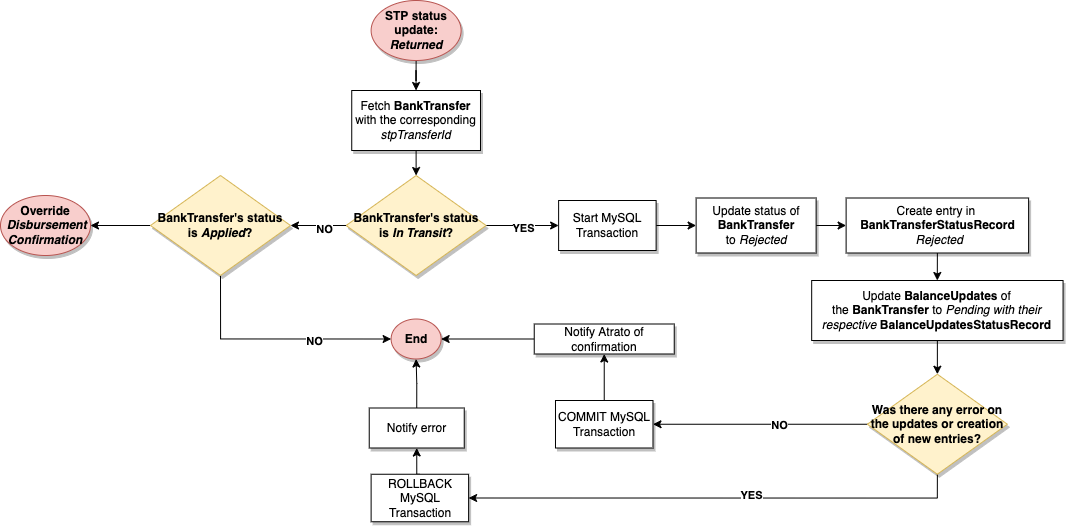
\includegraphics[scale = 0.4]{assets/diagrams/ReturnedStatus.png}
    \caption{Processing internal status of Balance Updates and Bank Transfer for Returned payment orders. Note the similarity with the Cancellation process}\label{fig:returned_status_update}
\end{figure}

//

In terms of mapping how the Balance Updates where related to the Bank Transfers the status worked perfectly, but to know the real balance of the store, multiple factors needed to be considered. The last Balance Update could indicate an actual balance of \$0.00, but if any previous Balance Update still had the status \textit{In transit}, then the real balance differed.\\ 

This complexity was not noted until a real edge-case, that was not previously considered, happend in production: for any Bank Transfer that was sent through STP a status update was expected. If none was recived, then the Balance Updates that generated that Bank Transfer will always remain with a status \textit{In transit}, and they will always appear as a pending movement for the store. If the bank transfer was cancelled, days after it was sent, then probably more Balance Updates and even Bank Transfers would have already been created by the time of the cancellation. If this was the case, then by the event of the next trigger for the Bank Transfer generation, all those previously generated Balance Updates would merge with the most recent ones to compose a new Bank Transfer, which was exactly the expected behaviour: to include in any new Bank Transfer all those Balance Updates that where still pending with the objetive of leaving none of them pending at all. As stated before, the status were very helpful to relate Balance Updates and Bank Transfers correctly, but the amount for the Bank Transfer could be complicated to decompose.\\

The ambiguity and the complex traceablity in the computation of the amount for every Bank Transfer led to the second approach: to keep the mapping and grouping of Balance Updates and Bank Transfers through their status, but consider always the store's actual balance for any new Bank Transfer. Furthermore, an additional change in the logic was required: unlike the first alternative, a Balance Update of type \textit{Disbursement} is now immediately generated once a Bank Transfer is sent, instead of waiting for STP's confirmation. With this approach, the store's actual balance, taken from the last Balance Update, is always considered for the amount of the next Bank Transfer. Once this newly generated Bank Transfer is sent, the \textit{Disbursement} Balance Update will be immediately generated, bringing the store's balance back to \textit{\$0.00}.\\ 

For stores with their balance system set up for immediate disbursements, unless an external event occurs such as possible cancelations or adjustments, their system will always be showing the following behaviour: an increase in the balance being affected by credit contributions and immediately a disbursement bringing the balance back down.\\


Additionally, if any of the Bank Transfers that were sent is later cancelled, a new Balance Update should be generated to compensate the changes in the store's balance already made by the \textit{Disbursement} Balance Update. This changes enable a much clearer understanding and breakdown of the store's balance in relation with every Bank Transfer that is sent. A cancellation of a Bank Transfer is very easy to understand, unlike with the previous appoach, where a cancellation would only bring back the status of the Balance Updates to \textit{pending}, and later assign them to a new Bank Transfer.\\ 

The change in the approach to this much simpler and undestandable algorithm was mainly triggered by some unexpected behaviour in STP's integration. The edge-case where no status update was received was never considered, and since its some responsibility of a third party then these actions rely outside of our area of control.\\ 

For such integrations and automated processes, it is of utmost importance to be able to track every trigger, action and result inside the processes occuring. By keeping a log of everything that is happening it is easier to monitor that everything is working as expected. Whenever an action is triggered, some very specific results should be happening, and when these results do not proceed as planned, then through these logs its easier to decid wether it is an error in the system that needs to be fixed or it is an error in the action that was triggered. Even for stores that do not have the balance system enabled, keeping  a log of how processes are interrupted is very important and these interruptions do not necessarily indicate an error, but on the contrary, that the system is disabled and will not proceed with the execution of the actions unless it is activated.

\section{Conclusion}

Automation in Atrato's business processes is a key factor for the scalability of current operations and even the final product for customers and partners. Now that the last step of the whole pipeline has been included in the automation, the next steps towards the growth that Atrato's customers and partners have been demanding should not be set back by operational load. To acomplish this, it was necessary to redefine and establish certain guidelines and procedurees for these operations. A process that is not clearly defined can and should not be automated, otherwise the outcomes could be very unpredictable. For this reason the first step, before even attempting to design and define the balance system for stores, was to define the current business process for the disbursements, analyze its limitations and define hould these could be addressed.\\

The whole commission and special promotions handling that was taking place in the commercial area could have been the rabbit hole that would prevent the successful automation of these processes. It was during the computation of the exact amount that needed to be disbursed per credit where most anomalies or differences where happening. By detaching the commission definition from the credit disbursement process, the latter could now be succesfully analyzed, addressed and automated.\\

By attempting to automate this process, as an indirect result, the whole disbursement operation was analyzed and redefined to become much simpler and well established. With the objective not to magnify the process' innefficiency, first it was necessary to define a very efficient pipeline and then proceed to automate and enhance this efficiency.\\

Furthermore, by integrating a third party service for the connection with the mexican digital banking system as part of the autmation of the balance system, possible external errors or misfunctions should also be considered. In other words, the system should be able reliable enough and should not interrupt internal processes when third party integrations are not working as expected. Every possible point of failure of the system was be thoroughly analyzed and the solutions were planned accordingly, such as the case where status updates on STP could not be received.\\

To be able to maintain a high level of traceablity throughout any store's balance system the use of Atrato's internal logging system was very helpful. Designing every controllers internal methods to implement the logger and always keep track of completed and interrupted processes with their corresponding payload for additional details was key for catching errors at early stages of development and even after deployment. Additionally, the use of query runners and MySQL Transactions is very useful for either completing a whole procedure or not at all. This left no uncomplete changes in the database and uncompleted processes or actions could be later addressed and retried.\\

Finally, the proposed solution to this manual and extensive process was successfully designed and developed: an automated system that could handle a store's balance and its changes through different internal and external triggers and actions to periodically or sistematically disburse the corresponding amount for the Atrato's partners' customers' purchases. Until now, one partner with three stores is already implementing this automation with real bank transfers. And a second partner, with more than 40 stores, is in the first process of validating their balance systems. More than 2.4 Million mexican pesos have already been processed through the system through 250+ bank transfers, the amount of which can be broken down into their corresponding individual Balance Updates.\\

These balance systems where integrated with existing business processes to enable a smooth and progressive transition into a fully automated system. By having the option of disabling and enabling these automations at any time, the whole process became completely backwards compatible in case it is necessary.\\


\section{Further Work}

A very interesting next approach to these balance systems would be to review the possibility to manage them not individually by store, but in a more general way by merchants. A merchant could have many stores, but it could be the same banking information and the same people managin all these stores. For these particular cases, it would be very convinient to manage all bank transfers from all these stores as part of one unified balance system. This balance will now be significant to the merchant itself, but keeping track of how every store contributed to the merchant's balance. This could add an additional layer of complexity to the whole system, but if designed appropiately, could also be very easy to handle and manage.\\ 

On the other hand, apart from the Dispersion service, STP provides a variety of services regarding the mexican digital banking system, not only for transfering money between banking accounts but also many interesting digital financial services that could possibly even open the opportunity for new products within Atrato's scope. As part of this integraiton, the connection was already established, making the implementation and integration of new services just a manner of further development that could be done.\\

Coming back to the development of the balance system, as part of the main objectives was to keep traceability of the processes at all times. Many of the design patterns and implementations used for these modules could be extended to further parts of Atrato's internal application. Designing systems where no processes are left incomplete and always accounting for external factors could lead to a very robust, reliable and scalable application. Atrato's next big challenges will not only involve further automations, but also building systems that support the scalability that is needed. Existing on-going business processes are going to need to stay up to date with Atrato's growth and start to be defined considering these factors in order to be able to be scaled without the need to grow the oprational team. A very efficient process with a very efficient team enhanced with the correct tools will be able to extend and keep the same high standard and top performance that is always expected.